\documentclass{standalone}
\usepackage{hsbcommon}
\makeatletter\AtBeginDocument{\@buildstepset{uk}}\makeatother
\begin{document}
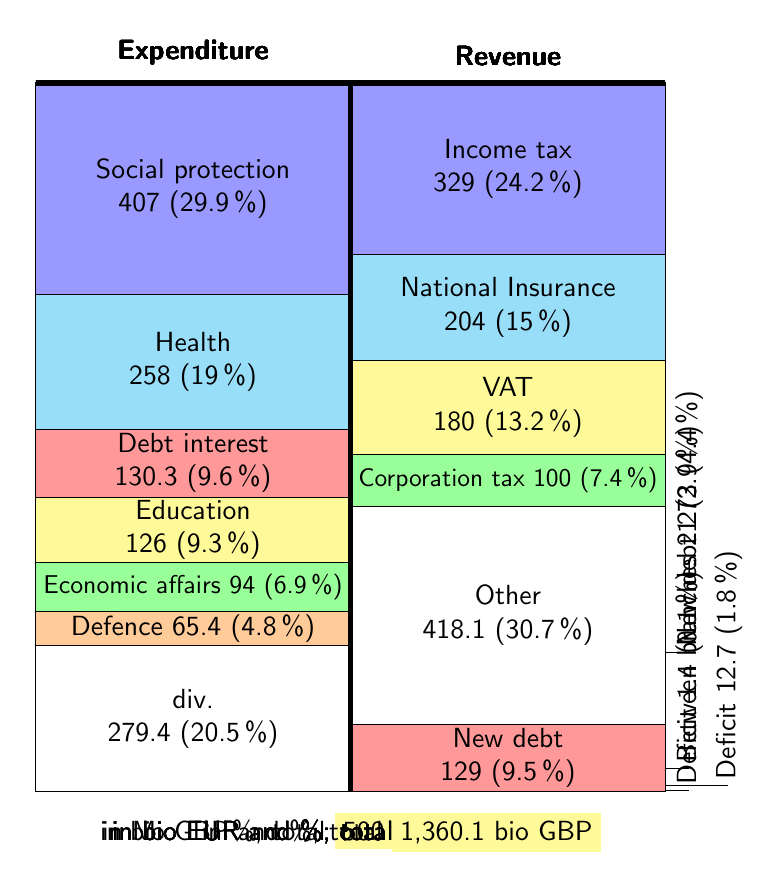
\begin{tikzpicture}
  %%% =================================================================
  %%% LAYOUT (local to this picture; works when \input elsewhere)
  %%% =================================================================
  \def\bdH{9}      % height of the taller bar in cm
  \def\bdW{4}      % bar width in cm
  \def\bdTwo{9}    % segments >= 9 % of the total: name and value on two lines
  \def\bdOne{4.5}  % segments >= 4.5 %: one line; smaller: label outside
  \def\bdRotate{1} % 1: small revenue labels rotated 90 degrees (narrow);
                   % 0: horizontal (use \\ in long names to break them)
  \def\bdShow{3}   % default for the values: 1 absolute, 2 percent, 3 both
                   % (can be overridden per chart: \budgetbars[2]{key})
  \tikzset{bd text/.style={font=\sffamily}}
  % \budgetdataset{key}{unit}{total}{expenditure list}{revenue list}
  % lists: value/color/name, ..., absolute values, stacked from the top down
  \newcommand\budgetdataset[5]{%
    \expandafter\def\csname bd-#1-unit\endcsname{#2}%
    \expandafter\def\csname bd-#1-total\endcsname{#3}%
    \expandafter\def\csname bd-#1-exp\endcsname{#4}%
    \expandafter\def\csname bd-#1-rev\endcsname{#5}}
  % caption below the T-account: #1 unit, #2 total
  \newcommand\bdcaption[2]{%
    \ifcase\bdmode\or in #1\or in \%\or in #1 and \%\fi;
    total \colorbox{yellow!40}{#2 #1}}
  % sum of a list into \bdsum
  \newcommand\bdsumof[1]{%
    \gdef\bdsum{0}%
    \foreach \v/\c/\n in #1 {\pgfmathsetmacro\bdt{\bdsum+\v}\xdef\bdsum{\bdt}}}
  % numbers as printed in the labels
  \newcommand\bdnum[1]{\pgfmathprintnumber[fixed, precision=1, 1000 sep={,}, assume math mode=true]{#1}}
  \newcommand\bdpctof[1]{%
    \pgfmathsetmacro\bdp{#1/\bdsidetotal*100}%
    \pgfmathprintnumber[fixed, precision=1, assume math mode=true]{\bdp}\,\%}
  % value of a segment according to the mode
  \newcommand\bdval[1]{%
    \ifcase\bdmode\or \bdnum{#1}\or \bdpctof{#1}\or \bdnum{#1} (\bdpctof{#1})\fi}
  % shrink a one-line label to the bar width if it is too wide
  \ifdefined\bdbox\else\newsavebox\bdbox\fi
  \newcommand\bdfit[1]{%
    \sbox\bdbox{#1}%
    \pgfmathsetlengthmacro\bdmax{\bdW cm-0.2cm}%
    \ifdim\wd\bdbox>\bdmax\resizebox{\bdmax}{!}{\usebox\bdbox}\else\usebox\bdbox\fi}
  % one segment: #1 x of bar, #2 bottom, #3 top (absolute values), #4 color,
  %              #5 name, #6 value, #7 side for outside labels (-1 left, 1 right)
  \newcommand\bdseg[7]{%
    \pgfmathsetmacro\bdyA{\bdH-#2/\bdscale*\bdH}%   stacked from the top down
    \pgfmathsetmacro\bdyB{\bdH-#3/\bdscale*\bdH}%
    \pgfmathsetmacro\bdyM{(\bdyA+\bdyB)/2}%
    \pgfmathsetmacro\bdpct{#6/\bdscale*100}%
    \draw[fill=#4, draw=black] (#1,\bdyA) rectangle (#1+\bdW,\bdyB);
    \ifdim \bdpct pt<\bdOne pt
      % small segment: no label on the expenditure side; on the revenue side
      % a label outside
      \ifnum#7>0
        \ifnum\bdRotate=1
          % rotated: each label rises from its leader, side by side
          \pgfmathsetmacro\bdxL{#1+\bdW+0.3+\bdcount*0.5}%
          \pgfmathtruncatemacro\bdc{\bdcount+1}\xdef\bdcount{\bdc}%
          \draw (#1+\bdW,\bdyM) -- (\bdxL,\bdyM)
            node[bd text, rotate=90, anchor=west, inner sep=2pt] {#5 \bdval{#6}};
        \else
          \pgfmathsetmacro\bdyL{min(\bdyM,\bdlast-0.45)}%
          \xdef\bdlast{\bdyL}%
          \draw (#1+\bdW,\bdyM) -- (#1+\bdW+0.3,\bdyL)
            node[bd text, anchor=west, align=left] {#5 \bdval{#6}};
        \fi
      \fi
    \else\ifdim \bdpct pt<\bdTwo pt
      \node[bd text] at (#1+\bdW/2,\bdyM) {\bdfit{#5 \bdval{#6}}};
    \else
      \node[bd text, align=center] at (#1+\bdW/2,\bdyM) {#5\\\bdval{#6}};
    \fi\fi
  }
  % one stacked bar: #1 x, #2 list, #3 side for outside labels, #4 heading
  \newcommand\bdbar[4]{%
    \gdef\bdlast{100}\gdef\bdcount{0}%
    \foreach \v/\c/\n [evaluate=\v as \bdtop using \bdbot+\v,
                       remember=\bdtop as \bdbot (initially 0)] in #2 {%
      \bdseg{#1}{\bdbot}{\bdtop}{\c}{\n}{\v}{#3}
    }
    \node[bd text, font=\sffamily\bfseries, anchor=south] at (#1+\bdW/2,\bdH+0.1) {#4};
  }
  % \budgetbars[mode]{key}: expenditure left, revenue right, as a T-account
  %   mode: 1 absolute values, 2 percent of each side's total, 3 both
  \newcommand\budgetbars[2][\bdShow]{%
    \edef\bdmode{#1}%
    \expandafter\let\expandafter\bdexp\csname bd-#2-exp\endcsname
    \expandafter\let\expandafter\bdrev\csname bd-#2-rev\endcsname
    \bdsumof{\bdexp}\let\bdsumE\bdsum
    \bdsumof{\bdrev}\let\bdsumR\bdsum
    \pgfmathsetmacro\bdscale{max(\bdsumE,\bdsumR)}%   both bars on one scale
    \let\bdsidetotal\bdsumE
    \bdbar{-\bdW}{\bdexp}{-1}{Expenditure}
    \let\bdsidetotal\bdsumR
    \bdbar{0}{\bdrev}{1}{Revenue}
    \draw[line width=2pt] (0,0) -- (0,\bdH);            % T-account
    \draw[line width=2pt] (-\bdW,\bdH) -- (\bdW,\bdH);
    \node[bd text, anchor=north] at (0,-0.15)
      {\bdcaption{\csname bd-#2-unit\endcsname}{\csname bd-#2-total\endcsname}};
  }

  %%% =================================================================
  %%% DATA (absolute values, stacked from the top down)
  %%% =================================================================
  % Example
  % Illustrative example: all shares are multiples of 5 %
  \budgetdataset{example}{bio EUR}{500}
    {175/blue!40/Social, 100/cyan!40/Defence, 50/yellow!40/Central fin.,
     50/red!40/Debt service, 25/green!40/Traffic, 100/white/div.}
    {350/blue!40/Taxes, 50/white/Other, 100/red!40/New debt}
  % Federal budget 2027, government draft (Drucksache 21/7300), bio Euro.
  % "Central fin." not verified; "div." and "Other" are remainders to 555.4.
  \budgetdataset{federal}{bio EUR}{555.4}
    {201.5/blue!40/Social, 109.7/cyan!40/Defence, 46.6/yellow!40/Central fin.,
     43.6/red!40/Debt service, 26.4/green!40/Traffic, 127.6/white/div.}
    {394.7/blue!40/Taxes, 42.0/white/Other, 118.7/red!40/New debt}
  % Land Bremen 2026, Mio Euro (Haushaltsportraet 2026/2027)
  \budgetdataset{bremen}{Mio EUR}{6,270}
    {1122.5/blue!40/Education, 1070.7/cyan!40/Social, 1071.9/yellow!40/Central fin.,
     612.8/green!40/Universities, 386/red!40/Debt service, 378.9/orange!40/Pensions,
     329.9/violet!40/Interior, 1297.3/white/div.}
    {3982/blue!40/Taxes, 919/cyan!40/Federal aid, 273/red!40/New debt,
     1096/white/div.}
  % United Kingdom 2025/26 (outturn), bio GBP.
  % Whole public sector (central and local government; there is no separate
  % social insurance budget). Spending: HM Treasury PESA 2026 via House of
  % Commons Library; receipts: House of Lords Library; borrowing: ONS.
  % "div." and "Other" are remainders to 1,360.1.
  \budgetdataset{uk}{bio GBP}{1,360.1}
    {407/blue!40/Social protection, 258/cyan!40/Health,
     130.3/red!40/Debt interest, 126/yellow!40/Education,
     94/green!40/Economic affairs, 65.4/orange!40/Defence, 279.4/white/div.}
    {329/blue!40/Income tax, 204/cyan!40/National Insurance, 180/yellow!40/VAT,
     100/green!40/Corporation tax, 418.1/white/Other, 129.0/red!40/New debt}     
  % French state budget 2027 draft (PLF), bio Euro, net of tax refunds
  \budgetdataset{france}{bio EUR}{474.9}
    {90.9/blue!40/Schools, 73.2/cyan!40/Defence, 72.9/red!40/Debt service,
     32.2/yellow!40/Solidarity, 32.1/green!40/Research, 22.5/orange!40/Housing,
     22.5/violet!40/Ecology, 128.6/white/div.}
    {318.4/blue!40/Taxes etc., 156.5/red!40/New debt}
  % German social insurance 2025, bio Euro (Destatis)
  \budgetdataset{desocial}{bio EUR}{937.5}
    {426.5/blue!40/Pensions, 352.4/cyan!40/Health, 73.8/yellow!40/Long-term care,
     84.8/white/div.}
    {771.5/blue!40/Contributions, 164.6/cyan!40/Federal funds, 1.4/red!40/Deficit}
  % French social security (basic schemes) 2027 draft (PLFSS), bio Euro.
  % Branch figures are gross: transfers between branches (21.0) appear as
  % spending of one branch and revenue of another.
  \budgetdataset{frsocial}{bio EUR}{717.4}
    {316.2/blue!40/Pensions, 277.1/cyan!40/Health, 60.2/yellow!40/Family,
     44.4/green!40/Autonomy, 19.5/white/div.}
    {328.2/blue!40/Contributions, 136.7/cyan!40/CSG, 116.2/yellow!40/Taxes,
     102.6/green!40/Other, 21.0/gray!25/Between branches, 12.7/red!40/Deficit}

  %%% =================================================================
  %%% PICTURE
  %%% =================================================================
  % fixed size for all steps (measured: rotated labels reach 5.05 on the right)
  \useasboundingbox (-4.1,-0.95) rectangle (5.1,9.7);
  % optional [1|2|3] overrides \bdShow: 1 absolute, 2 percent, 3 both
  \ifstep{example}{\budgetbars[2]{example}}
  \ifstep{1,federal}{\budgetbars{federal}}
  \ifstep{2,bremen}{\budgetbars{bremen}}
  \ifstep{3,france}{\budgetbars{france}}
  \ifstep{4,desocial}{\budgetbars{desocial}}
  \ifstep{5,frsocial}{\budgetbars{frsocial}}
  \ifstep{6,uk}{\budgetbars{uk}}
\end{tikzpicture}
\end{document}